\chapter{What a compatible explanation must contain}
\label{rf:entry}

The access problem has a useful next form. Instead of asking only whether two
known mechanisms can be distinguished, ask what \emph{every} compatible
explanation must contain. The answer may be a minimum number of classical
states, a sufficiently large preparation resource, or sustained dissipation.
These are different physical quantities. Their inference requires different
experimental access, and they must not be collapsed into a universal scalar
``information cap.''

The following chapters establish complementary boundaries of this question.
A robust nonnegative-factorization argument turns one preparation and one
repeated channel into a finite-data hierarchy of classical state requirements.
Erlang observation clocks give another route: finite measured probabilities
certify a spectral obstruction without estimating exact hidden poles or
bounding unseen transition rates. This certificate works at lower coherence
than the explicit hierarchy example, but its sufficient record bound is much
larger.

A constructive converse prevents overinterpretation. Finite fresh-reset
prepare--wait--read records with continuous target probabilities can be approximated arbitrarily well by finite,
irreducible, detailed-balance classical models when hidden dimension, rates and
preparation resources are unrestricted. The construction retains timestamps
and accommodates adaptive choices between reset trials. It does not reproduce
arbitrary interventions within a persistent trajectory. Its explicit state and
preparation requirements explain why an unrestricted classical null cannot be
rejected uniformly from that restricted access.

Stationary pair observations impose additional structure. Reversible Markov
autocorrelations are nonnegative mixtures of decaying exponentials. A measured
departure from this class yields a quantitative preparation--housekeeping
requirement; stationary preparation strengthens it to a sustained entropy-rate
bound. Exact dual certificates turn uncertain finite observations into such
requirements without selecting a hidden network architecture.

\begin{center}
\begin{tabular}{p{0.29\textwidth}p{0.30\textwidth}p{0.30\textwidth}}
\toprule
Access and premise & Certified conclusion & Essential qualification\\
\midrule
Repeated common channel, fixed preparation and readout & Minimum classical state count & Hidden control and detector memory count as states\\
Finite reset records, unrestricted hidden resources & Constructive classical approximation & No nontrivial uniform test against the full null\\
Stationary noninvasive binary pairs & Entropy-production lower bound & Ordinary reversal and thermodynamic embedding required\\
Nonstationary pairs and a preparation budget & Preparation--housekeeping tradeoff & Reference mean cannot be inferred from transient mean\\
\bottomrule
\end{tabular}
\end{center}

This is an extension of the common access contract, not a replacement for
established system identification, positive realization or stochastic
thermodynamics. The useful contribution is an explicit chain from observations
to requirements on all members of a declared explanatory class, with exact
countermodels where that chain cannot proceed. Candidate historical novelty,
mathematical verification and laboratory validation remain separate questions.


\begin{figure}[ht]
\centering
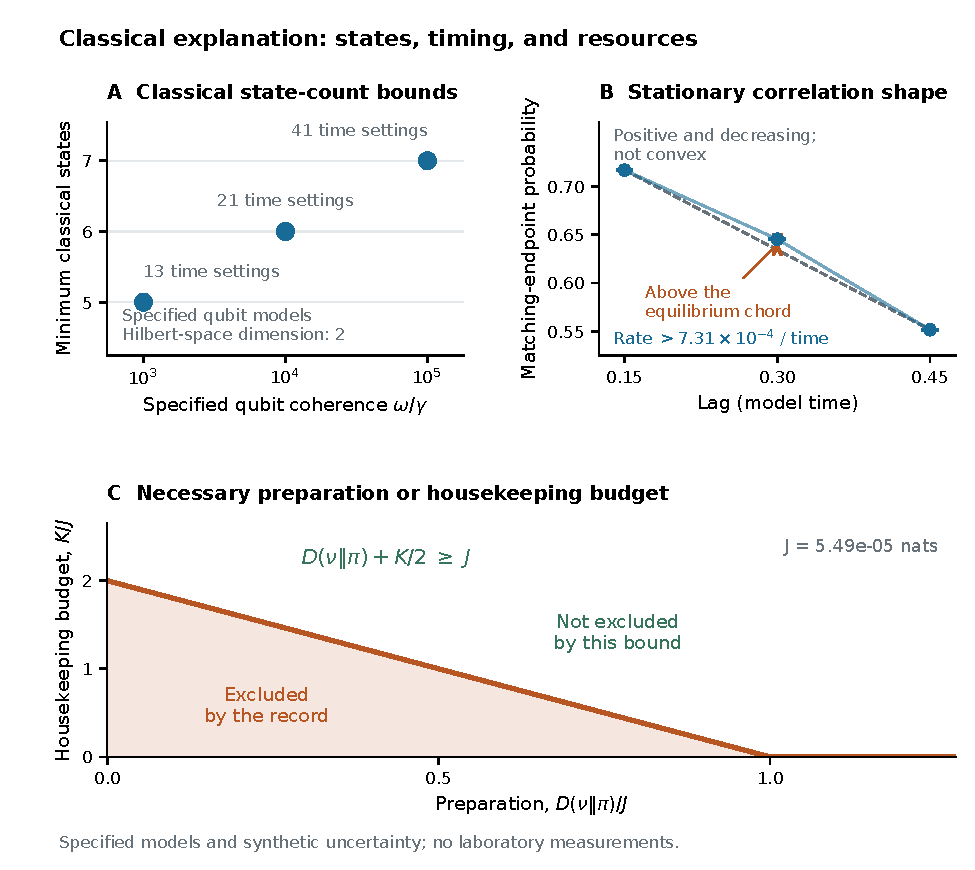
\includegraphics[width=\textwidth]{figures/realization_frontier.pdf}
\caption{Three types of requirements on a classical explanation.
(A) Specified finite-noise qubit examples force increasing classical state
counts under one repeated-channel contract; these points are not an optimized
coherence threshold. (B) The stationary ring example has positive decreasing
agreement probabilities but violates reversible convex decay. Error bars show
a synthetic uncertainty box. (C) A certified record separation $J$ excludes
preparation--housekeeping budgets below $D+K/2=J$. The region above the line
is merely not excluded by this bound; attainability is not asserted.
All panels are model-based and require their respective access assumptions.}
\label{rf:overview-figure}
\end{figure}
